
\chapter{Introducción}
%% Este 'capitulo' o sección del documento no  numera ni secciones o subsecciones, se utiliza el esquema de libro para ordenar la información

La conservación de la flora y fauna en el planeta, especialmente de las especies en peligro de extinción, se ha convertido en una problemática social apremiante. Cada año, la lista de especies amenazadas o extintas sigue creciendo, lo cual plantea una preocupación apremiante para mantener el equilibrio de los ecosistemas \cite{1}. A pesar de los esfuerzos realizados con técnicas y métodos tradicionales y actuales para el monitoreo de estas especies, existen desventajas significativas que limitan su eficacia. Por lo tanto, se requiere una innovación en el enfoque de monitoreo para mejorar la protección de estas especies vulnerables.\\
En la actualidad, los métodos de monitoreo tradicionales, como censos manuales y observación directa, son costosos, lentos y pueden ser invasivos ya que requieren la intervención del hábitat natural causando estrés y alterando el comportamiento natural de la especie animal \cite{2}. Asimismo, la falta de cobertura continua y la complicada accesibilidad a áreas remotas, dificultan la recopilación de datos precisos y en tiempo real, lo cual puede dificultar la toma de decisiones informadas para su protección \cite{3}. \\
Ante este panorama, surge la necesidad de explorar nuevas alternativas tecnológicas que permitan un monitoreo más efectivo y menos invasivo. Una solución prometedora es el uso de una red inalámbrica de sensores (WSN, por sus siglas en inglés) ubicados estratégicamente en diferentes puntos del hábitat natural de la especie en estudio \cite{4}. Estos sensores pueden recopilar datos sobre el comportamiento, ubicación y otros parámetros de interés de la especie, sin interferir con su comportamiento natural como en el trabajo de TigerCENSE \cite{5}, donde se utiliza una WSN con un sensor infrarrojo pasivo para capturar imágenes de un tigre en peligro de extinción sin interferir con su comportamiento natural.\\
Algo semejante ocurre con el uso de drones como vehículos aéreos para la recolección de la información recopilada por los sensores de la WSN al ofrecer ventajas significativas en términos de acceso a áreas remotas, velocidad y precisión en la recopilación de datos \cite{6}. Los drones pueden sobrevolar el hábitat para recolectar los datos de manera no invasiva y transportarlos a una estación base (BS), brindando a los biólogos de campo una visión detallada de la situación de la especie que desean preservar \cite{7}.\\
Sin embargo, los sistemas de monitoreo que utilizan un solo dron presentan desventajas significativas en términos de consumo de energía, cobertura y conexión remota. Estos sistemas pueden ser limitados en la duración de su tiempo de vuelo y alcance, lo que puede dificultar el monitoreo continuo y en tiempo real de las especies amenazadas. Agregando que en áreas remotas o de difícil acceso, la conexión remota puede ser insuficiente para transmitir los datos de manera óptima \cite{8}.
Por anterior, en este documento se abordará de manera integral la propuesta de una solución innovadora para el monitoreo de especies en peligro de extinción. Comenzando por explorar el planteamiento del problema, destacando las limitaciones de los métodos actuales, y posteriormente, justificando la urgencia de adoptar enfoques más efectivos. La propuesta de solución se desarrollará mediante la presentación de subsistemas, como el enjambres de drones, la redes inalámbricas de sensores (WSN) y su integración. Además, se delinearan los objetivos y alcances para proporcionar un marco claro de los logros esperados. Se explorará el estado del arte y el marco teórico, contextualizando la investigación en el panorama científico actual. Luego, se realizará un análisis detallado de los componentes clave, desde sensores y drones hasta los servicios en la nube. También se abordará el diseño de los elementos vistos en el análisis, presentando las estructuras físicas y lógicas de los drones, el enjambre y el dominio en la nube. Finalmente, se examinarán los resultados de pruebas en simulación y esquemas de vuelo, preparando el terreno para las validaciones en el escenario de pruebas.

%\newpage
\chapter{Planteamiento del Problema}

La protección de las especies en peligro de extinción y la preservación de la biodiversidad son temas críticos que preocupan a la comunidad científica y a la sociedad en general \cite{15}. En este sentido, los biólogos de campo han implementado técnicas de monitoreo y seguimiento para evaluar la salud y el tamaño de la población de la especie, así como la calidad de su hábitat \cite{16}. Una de estas técnicas es la observación directa, que consiste en la observación visual de las especies en su entorno natural \cite{17}. Si bien, esta técnica permite obtener datos detallados sobre el comportamiento y la interacción de las especies, presenta limitaciones en términos de cobertura espacial y temporal, ya que depende de la presencia de los biólogos en el terreno. Esto dificulta su implementación en regiones remotas o de difícil acceso, conllevando riesgos y costos significativos en términos de recursos humanos y logísticos \cite{18}, y ocasionando perturbaciones que pueden generar efectos negativos en la especie y en su hábitat \cite{19}.\\
Otra técnica utilizada es el monitoreo acústico, que se basa en el registro y análisis de los sonidos emitidos por las especies. Permite obtener información sobre la actividad, la comunicación y la distribución espacial de las especies. Sin embargo, la identificación precisa de las especies a través de los sonidos puede ser compleja, especialmente cuando hay varias especies presentes en un área \cite{20}. Agregando que las condiciones ambientales pueden afectar la calidad de los datos acústicos debido al ruido de fondo.\\
El monitoreo por medio de rastreo y seguimiento satelital es otra técnica empleada, que permite obtener datos sobre la ubicación y los movimientos de las especies a través de dispositivos de rastreo satelital. Esto proporciona información detallada sobre los patrones de migración, la distribución espacial y la interacción de las especies con su entorno. Sin embargo, esta técnica puede resultar costosa debido al equipo y los servicios de satélite necesarios, y también puede tener limitaciones en términos de precisión y resolución espacial \cite{21}.\\
Aparte de estas técnicas, también se ha empleado el monitoreo con un solo dron para capturar imágenes y datos desde el aire. No obstante, esta técnica exhibe importantes desventajas técnicas. Por un lado, se encuentra restringida en cuanto a la cobertura espacial debido al alcance y autonomía limitados del dron. Además, se necesita contar con un piloto experto para operar el dron de forma segura. Asimismo, recolectar datos desde múltiples perspectivas o ángulos diferentes puede resultar complicado con un solo dron \cite{22}.\\
En vista de la necesidad imperante de desarrollar un sistema de monitoreo remoto para especies en peligro de extinción, se plantea la aplicación de redes inalámbricas de sensores (WSN) como una solución tecnológica con potencial prometedor. Esta propuesta busca permitir la recopilación de datos precisos sobre las especies en cuestión, al tiempo que minimiza las perturbaciones en su hábitat y reduce los riesgos asociados para los biólogos de campo. Sin embargo, la implementación de WSN en entornos caracterizados por su difícil acceso y condiciones remotas plantea desafíos particulares. Entre ellos se encuentran los problemas de comunicación en áreas aisladas, la necesidad de establecer una conectividad efectiva entre la WSN y los drones encargados de la recolección de datos, así como la garantía de una transmisión de información confiable en condiciones ambientales adversas \cite{22.2}.
Ante estos desafíos, el enfoque tecnológico de la telemática emerge como una solución potencialmente efectiva y viable para superar las limitaciones y maximizar los beneficios del monitoreo remoto de especies en peligro de extinción.\\
Basándonos en las consideraciones expuestas, la pregunta de investigación que orientará este trabajo es la siguiente: ¿Cómo se puede implementar un sistema de monitoreo remoto de especies en peligro de extinción utilizando una red de sensores inalámbrica capaz de transmitir datos a un enjambre de drones que utilice una estrategia de recolección de datos eficiente?

%%%%%%%%%%%%%%%
%\newpage
\chapter{Justificación}

La protección de las especies en peligro de extinción es crucial para garantizar la supervivencia de la biodiversidad del planeta. Cada especie tiene un valor intrínseco y único, y su pérdida representa una disminución irreparable de la diversidad biológica del ecosistema \cite{9}. La biodiversidad es esencial para el equilibrio y la estabilidad de los ecosistemas, ya que cada especie cumple un papel importante en su funcionamiento. Agregando que, el valor intrínseco de estas especies también puede tener un valor económico. Por ejemplo, pueden ser utilizadas como recursos para la investigación científica, lo que contribuye al avance del conocimiento científico y tecnológico. Del mismo modo, su conservación puede tener beneficios para el turismo ecológico, generando empleo y oportunidades económicas en las comunidades locales \cite{10}. \\
La protección de las especies animales que se encuentran en esta situación también tiene beneficios indirectos para el medio ambiente y la sociedad en su conjunto. La conservación de estas especies puede contribuir a la preservación de los ecosistemas y los servicios ambientales que estos proporcionan, como la regulación del clima, la polinización de cultivos y la purificación del agua. La pérdida de una especie puede tener un efecto dominó en el ecosistema, afectando a otras especies y a la misma funcionalidad del ecosistema en su conjunto \cite{11}. De igual forma, la pérdida de biodiversidad puede tener consecuencias negativas para la salud humana y la calidad de vida, dado que la biodiversidad está estrechamente relacionada con la salud de los ecosistemas y, por ende, con la salud de las personas \cite{12}. La pérdida de especies puede afectar la disponibilidad de alimentos, medicinas y otros recursos naturales que son esenciales para la subsistencia y el bienestar de las comunidades humanas \cite{13}. \\
Por lo tanto, es fundamental contar con un sistema de monitoreo eficiente y preciso para los animales que se encuentran en riesgo de una posible extinción \cite{14}. Un sistema de monitoreo mediante una red inalámbrica de sensores puede proporcionar datos y observaciones precisas sobre el comportamiento, la distribución y la salud de estas especies, lo que permite a los expertos tomar decisiones informadas y estratégicas para su conservación. Este tipo de sistema de monitoreo puede ser una herramienta valiosa en los esfuerzos de conservación de estas especies, garantizando su supervivencia y contribuyendo a la protección de la biodiversidad y la estabilidad de las comunidades humanas que dependen de ella.


 \begin{figure} [h]
     \centering
     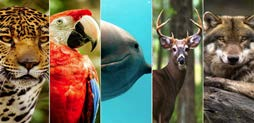
\includegraphics[width=0.5\linewidth]{imagenes/img1_ejemplos_especies_peligro_extincion.jpg}
     \caption{Ejemplos de especies en peligro de extinción.}
     \label{fig:enter-label}
 \end{figure}
%%%%%%%%%%%%%%%%%%%%
\newpage
\chapter{Propuesta de Solución}
Las etapas en las que se divide esta propuesta de solución se describen de forma general a continuación:

\section{Subsistema 1: Enjambre de Drones y Estación Base}
El uso de enjambres de drones en la biología de campo ha emergido como una innovadora y prometedora herramienta para la recolección de datos en áreas remotas y de difícil acceso, facilitando el monitoreo y estudio de la biodiversidad en estos entornos \cite{23}. En vista de que, a menudo los biólogos de campo enfrentan largos y agotadores recorridos para acceder a áreas de estudio, implicando un gran costo en términos de tiempo, esfuerzo físico y recursos \cite{24}. A su vez, la presencia humana en áreas naturales puede perturbar a las especies en peligro de extinción y afectar negativamente a los hábitats frágiles. Es por esto que se propone el uso de un enjambre de drones que pueda volar en formación hacia una red inalámbrica de sensores (WSN) con el fin de recolectar datos relevantes sobre la especie y su hábitat.\\
Las ventajas del empleo de un enjambre, en comparación con un solo dron, son diversas. En primer lugar, la robustez del enjambre es superior \cite{25}, ya que si uno de los drones falla o presenta algún problema, los demás drones pueden continuar con el proceso de recolección de datos, asegurando la continuidad de la operación sin interrupciones significativas. En segundo lugar, la capacidad de recolección de datos se ve incrementada considerablemente al utilizar un enjambre en lugar de un solo dron \cite{26}. Cada dron del enjambre puede recolectar información simultáneamente, lo que permite cubrir un área mayor en menos tiempo y almacenar una cantidad considerablemente mayor de datos. Esto es especialmente beneficioso en estudios de biología de campo donde se requiere recolectar una gran cantidad de información para obtener resultados confiables y de forma más rápida.\\
Otra ventaja destacada del uso de enjambres de drones es su capacidad para enfrentar condiciones adversas \cite{27}, como ráfagas de viento. Debido a la distribución y coordinación entre los drones, el enjambre puede compensar mejor los efectos del viento, manteniendo una posición y estabilidad más robustas durante el vuelo. Esto garantiza una mayor precisión en la recolección de datos y reduce el riesgo de errores o pérdidas de información debido a las condiciones climáticas.\\
La arquitectura del sistema propuesto consiste en una combinación de tecnologías y componentes clave. En el enjambre de drones, cada dron estará equipado con transceptores inalámbricos que permitirán la comunicación entre ellos y con la red de sensores. Para asegurar la eficiencia en la recolección de datos, se utilizarán algoritmos de coordinación y control que permitirán la sincronización de los drones y la asignación de tareas específicas a cada uno. Este proyecto no contempla la programación del enjambre de drones, solo la implementación de drones coordinados autónomos.\\
En cuanto a los transceptores, se considerarán diferentes opciones tecnológicas, como WiFi o LoRa, en función de los requerimientos del sistema. Estas tecnologías permitirán la comunicación bidireccional entre los drones y la red de sensores, facilitando la transferencia de datos y comandos de control.


\begin{figure}[h]
    \centering
    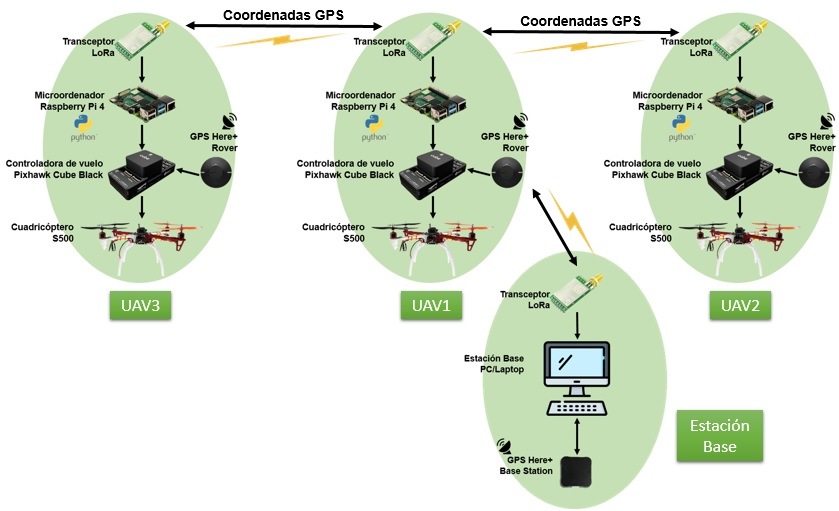
\includegraphics[width=0.9\linewidth]{imagenes/img2_disenho_drones_coordinados.jpg}
    \caption{Diseño y arquitectura del sistema de tres drones coordinados.}
    \label{fig:enter-label}
\end{figure}
\newpage
\section{Subsistema 2: WSN y el Monitoreo Remoto en Especies en Peligro de
Extinción}
En esta etapa, se propone el diseño de una red inalámbrica de sensores (WSN) de tipo clusterizada basada en un modelo matemático capaz de predecir el consumo energético de la red, determinar el número máximo de nodos y estimar la capacidad de transmisión de datos.
Una vez realizado el análisis, se procederá a implementar la WSN. Para ello, se seleccionarán cuidadosamente los dispositivos y el sistema de comunicaciones más adecuado, teniendo en cuenta la compatibilidad con el subsistema de comunicación del enjambre de drones. Además, se desarrollar á una interfaz temporal de adquisición de datos para monitorear, identificar y procesar la información proveniente de los animales.
Por otro lado, se llevará a cabo una investigación para adquirir o desarrollar los sensores y dispositivos apropiados para la especie seleccionada. Se considerarán los tipos de datos más relevantes para el monitoreo, según la experiencia de los expertos en el campo. Entre estos datos se encuentran las coordenadas GPS del animal durante un periodo de tiempo en caso de utilizar collares, así como las condiciones ambientales obtenidas directamente de un sensor de temperatura a la WSN.
En la parte del monitoreo, se empleará exclusivamente el sistema de posicionamiento global (GPS) para geolocalizar a los animales. Las posiciones registradas se almacenarán en tarjetas de memoria SD dentro de los sensores líderes de cada clúster. Durante los vuelos del enjambre de drones para recolectar información, los datos se enviarán junto con la información de la temperatura y el video de las cámaras trampa.

\begin{figure}[h]
    \centering
    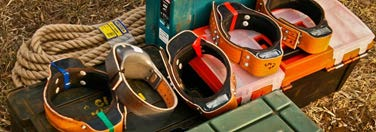
\includegraphics[width=0.8\linewidth]{imagenes/img3_ejemplos_collares.jpg}
    \caption{Ejemplos de tipos de collares de seguimiento de animales.}
    \label{fig:enter-label}
\end{figure}

\noindent La arquitectura de los clúster heads, encargados de coordinar la comunicación entre los drones y la WSN, se diseñará considerando la selección de una tecnología específica, la cual se determinar á en etapas posteriores del proyecto. Algunas alternativas a considerar podrían ser el uso de dispositivos Raspberry Pi, Arduino o módulos de comunicación especializados.

\section{Subsistema 3: Integración, Esquemas y Entorno de Visualización}
En esta etapa se planea integrar los dos subsistemas anteriores mediante un funcionamiento como se puede ver en las Figuras \hyperref[figura4]{4.3a} y \hyperref[figura4]{4.3b} donde se pone de ejemplo el monitoreo de jaguares (el escogimiento de la especie a monitorear dependerá del análisis que se realizará con biólogos de campo). En la Figura \hyperref[figura4]{4.3a}, la WSN se encarga de recopilar los datos de la cámara trampa, del sensor de temperatura y de los GPS que llevará la especie animal en un dispositivo de seguimiento que dependerá del tamaño de la especie que se planee monitorear. En la Figura \hyperref[figura4]{4.3b}, el enjambre de drones se dirigirá a la WSN para recolectar todos estos datos y ser llevados a la BS.


\begin{figure}[h]
\centering
    \begin{subfigure}
        \centering
        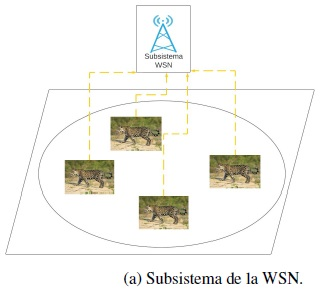
\includegraphics[width=0.45\linewidth]{imagenes/fig4_a.jpg}
        %\caption{Subsistema de la WSN.}
    \end{subfigure}    
    \hfill
    \begin{subfigure}
        \centering
        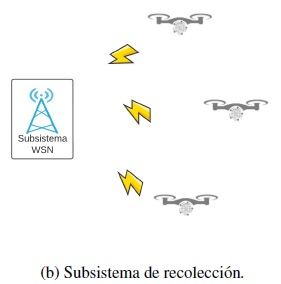
\includegraphics[width=0.45\linewidth]{imagenes/fig4_b.jpg}
        %\caption{Subsistema de recolección.}
    \end{subfigure}
    \caption{Funcionamiento del sistema.}
    \label{figura4}
\end{figure}


\noindent Como parte de la propuesta de solución, se llevará a cabo una comparación energética y de tiempo de vuelo del enjambre de drones entre dos esquemas de recolección de datos.\\
En el primer esquema propuesto, cada uno de los drones del enjambre se dirigirá de manera individual hacia cada WSN con el propósito de recolectar los tres tipos de información almacenados: video, coordenadas GPS y temperatura ambiental. Esta configuración se representa visualmente en la Figura \hyperref[figura5]{4.4}.
\begin{figure}[h]
    \centering
    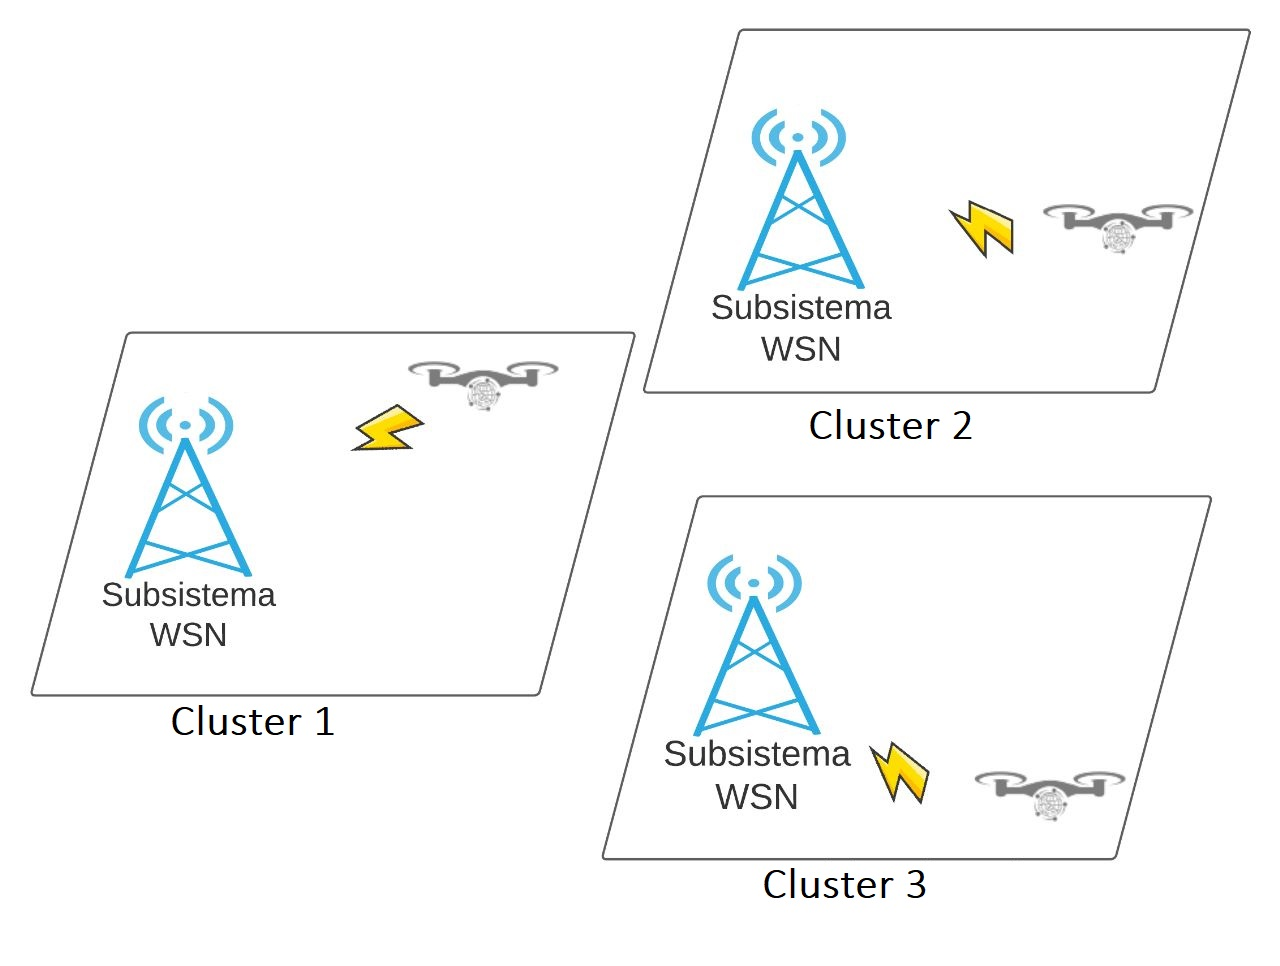
\includegraphics[width=0.5\linewidth]{imagenes/img5_recoleccion_enajmbre.jpg}
    \caption{Primer esquema de recolección (enjambre separado).}
    \label{figura5}
\end{figure}
\newpage
\noindent En el segundo esquema, los drones del enjambre se dirigirán conjuntamente a cada WSN, sin embargo, a cada dron se le asignará la responsabilidad de recolectar un tipo específico de información. De esta forma, un dron se encargará exclusivamente de recolectar video, otro se encargará de recopilar las coordenadas GPS, y el tercer dron se focalizará en la obtención de datos relacionados con temperatura ambiental. Este enfoque de asignación de tareas se repetirá en cada WSN, tal como se ilustra en la Figura \hyperref[figura6]{4.5}.

\begin{figure}[h]
    \centering
    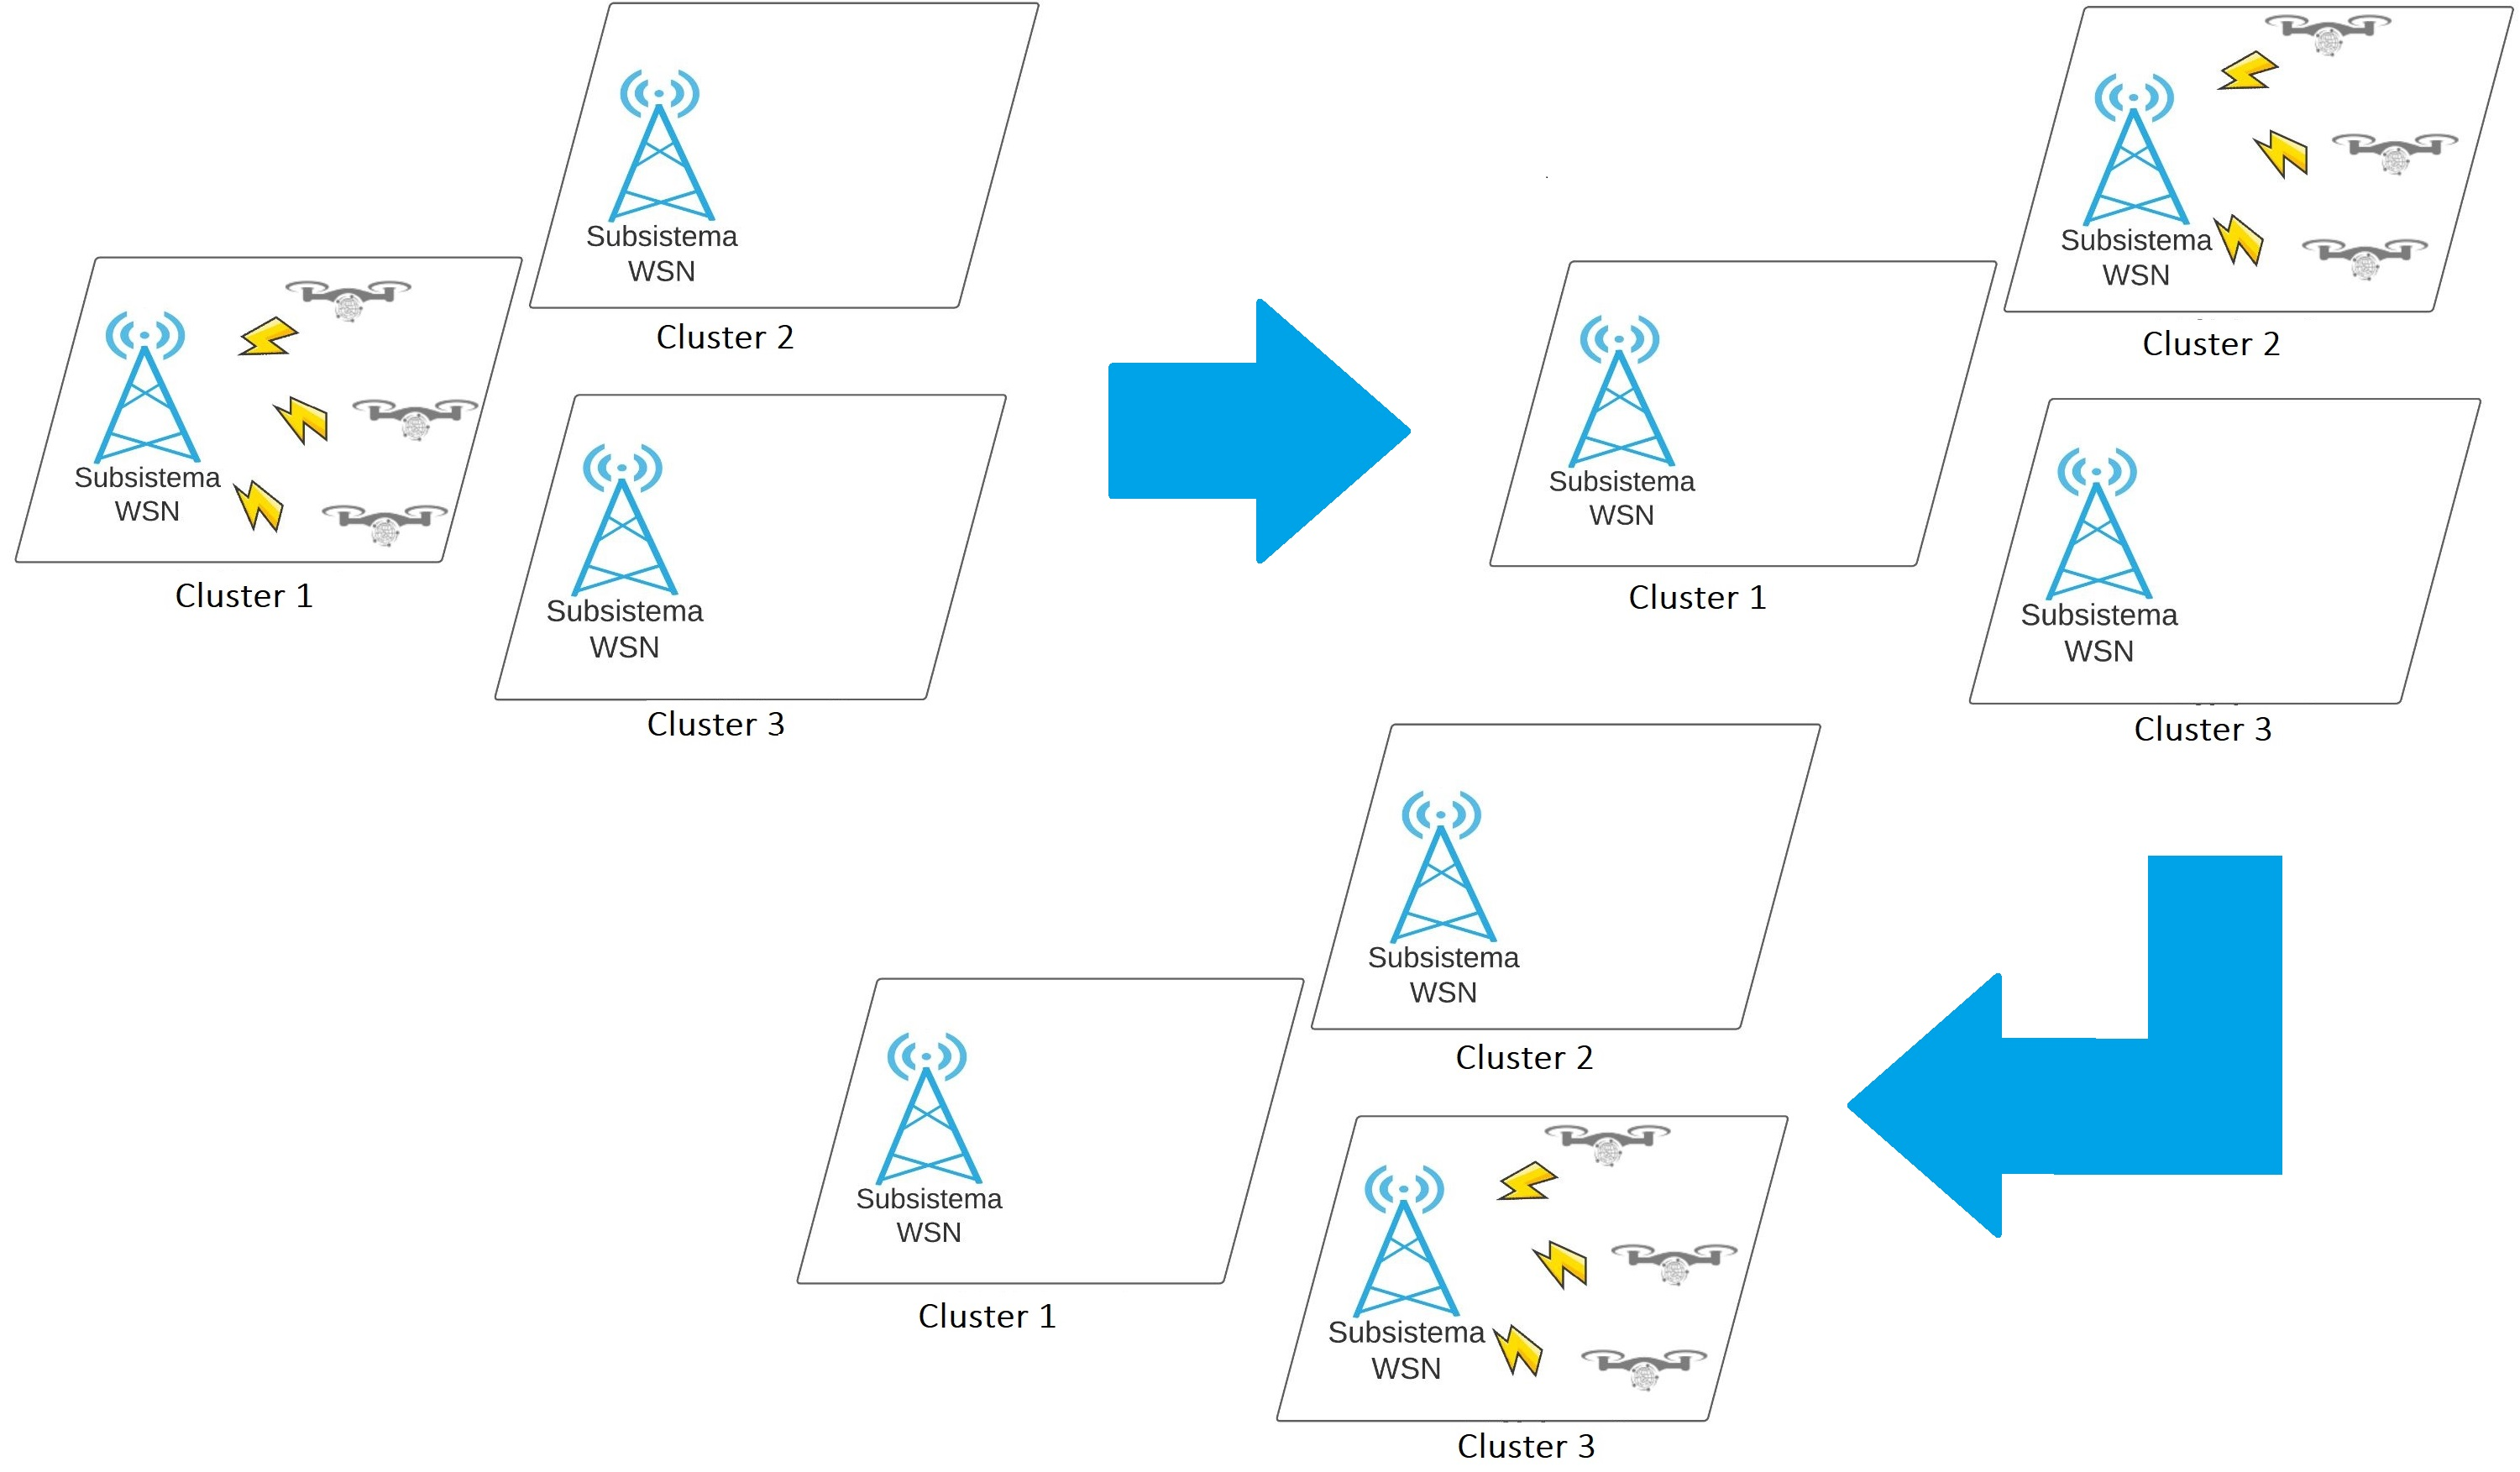
\includegraphics[width=0.7\linewidth]{imagenes/img6_segundo_esquema_recoleccion.jpg}
    \caption{Segundo esquema de recolección (enjambre en conjunto).}
    \label{figura6}
\end{figure}
\newpage
\noindent La comparación entre estos dos esquemas se realizará a través de un análisis matemático que proporcionará información valiosa para determinar cuál de ellos es más eficiente y adecuado para la propuesta de solución de este trabajo, al realizar mediciones y análisis precisos de la energía consumida por cada dron durante la recolección de datos, así como el tiempo requerido para completar la tarea en cada esquema.
Por todo esto, el uso de este enjambre presentará numerosas ventajas. En primer lugar, permitir á a los biólogos de campo recolectar datos de manera más rápida y efectiva, al cubrir grandes áreas en poco tiempo y acceder a lugares que serían difíciles o peligrosos para los humanos. En segunda instancia, reducirá la perturbación a los hábitats naturales, ya que los drones pueden sobrevolar el hábitat a una gran altura para diluir el ruido que sus motores generan; además, no alteran la vegetación y minimizan la presencia humana en las áreas de estudio. Esto es especialmente importante en el caso de especies que se encuentran en un alto riesgo de desaparecer, donde cualquier perturbación adicional puede tener un impacto negativo en su comportamiento y hábitat. Otra ventaja del uso de enjambres de drones es la posibilidad de programar rutas de vuelo preestablecidas, permitiendo así una mayor precisión en la recolección de datos al seguir una ruta específica para recolectar datos y eliminar la necesidad de contar con un operador de drones \cite{28}.
Una vez que el enjambre ha recopilado los datos, es necesario contar con un entorno adecuado para su análisis y almacenamiento. En este sentido, se propone implementar una solución basada en una base de datos en la nube, que permitirá disponer de un sistema distribuido de fácil acceso, el cual contará con:


\begin{itemize}
    \item La apertura de una aplicación web que brinde la posibilidad a especialistas de visualizar los datos ya procesados.
    \item  La creación de distintos perfiles de usuario, con acceso diferenciado a los datos almacenados y no analizados.
    \item Acceso a archivos multimedia como vídeos, imágenes y audios recabados, que estarán almacenados en una base de datos.
\end{itemize}

\noindent Esta infraestructura garantizará una gestión eficiente de los datos y la seguridad de los mismos para su posterior disponibilidad en el análisis y consulta.
Para lograrlo, se propone utilizar los servicios de AWS (Amazon Web Services), los cuales ofrecen una amplia gama de herramientas y capacidades. A continuación, se mencionan algunos servicios de AWS que se plantea utilizar:

\begin{itemize}
    \item \textbf{Amazon Cognito: }Un servicio de autenticación y autorización para las aplicaciones web y móviles \cite{29}. Este servicio permitirá autenticar y autorizar los accesos a la información, asignando a cada usuario un nivel de acceso específico.
    \item \textbf{Amazon S3: }Un servicio de almacenamiento de datos que ofrece escalabilidad, disponibilidad de datos, seguridad y rendimiento líderes en el sector. Permite almacenar y proteger cualquier cantidad de datos para diversos casos de uso, como lagos de datos, aplicaciones nativas en la nube y aplicaciones móviles \cite{30}. Se utilizará para el almacenamiento de archivos multimedia, tales como los vídeos de las cámaras trampa.
    \item \textbf{Amazon DynamoDB:} Un servicio de base de datos NoSQL totalmente administrado que proporciona un desempeño rápido y predecible con una escalabilidad perfecta. Permite crear tablas de base de datos para almacenar y recuperar cualquier cantidad de datos y atender cualquier nivel de tráfico de solicitudes. Al distribuir automáticamente los datos y el tráfico de la tabla entre un número suficiente de servidores para gestionar la capacidad de solicitud especificada por el cliente y la cantidad de datos almacenados, al mismo tiempo que mantiene un desempeño rápido y constante \cite{31}. Se utilizará para la administración de los archivos multimedia e información adicional sobre los datos recabados y procesados. Usando la API GraphQL, para la búsqueda de información dentro de DynamoDB, mediante AppSync; La utilización de la API GraphQL es una opción para llevar a cabo búsquedas de información dentro de DynamoDB a través de AppSync, que es un servicio proporcionado por AWS específicamente diseñado para ejecutar consultas sobre la información almacenada en la base de datos.
    \item \textbf{AWS Amplify:} Una solución completa que permite a los desarrolladores web y móviles crear, enviar y alojar aplicaciones de pila completa en AWS de forma sencilla \cite{32}. Facilitará la interconexión entre las bases de datos, el Back-end y el Front-end, sin requerir experiencia en la nube. Además, se puede considerar la creación de una página web utilizando HTML5, CSS y JavaScript.

\end{itemize}

\begin{figure}[h]
    \centering
    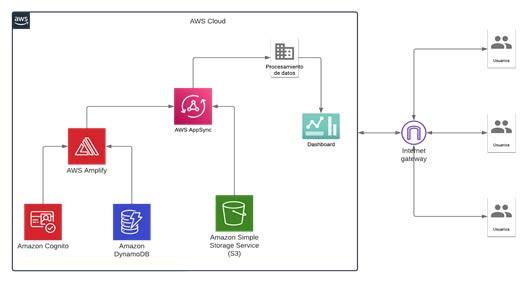
\includegraphics[width=0.8\linewidth]{imagenes/img7_arquitectura_propuesta_aws.jpg}
    \caption{Arquitectura de propuesta para el almacenamiento y procesamiento de datos.}
    \label{fig:enter-label}
\end{figure}

%%%%%%%%%%%%%%%%%

\chapter{Objetivos}
\section{Objetivo General}
Implementar un sistema integral de recolección, almacenamiento y visualización de información relevante para el monitoreo de una especie en peligro de extinción, la cual se determinará en etapas posteriores del proyecto en colaboración con expertos en conservación y protección animal.
Para ello, se llevará a cabo el diseño y reprogramación del enjambre de drones, así como el diseño e implementación de la WSN y del servicio en la nube, eligiendo el esquema de recolección de acuerdo al modelo energético.

\section{Objetivos Particulares}
\subsection{Proyecto Terminal 1}
\begin{itemize}
    \item Analizar los componentes necesarios para el subsistema de la WSN, así como el tipo de red y los métodos de formación y transmisión de datos entre los sensores más adecuados, así como desarrollar el modelo y simulación adecuado y para la caracterización del desempeño de la red.
    \item Analizar y elegir los componentes del subsistema de adquisición de datos de la WSN y enjambre, así como de la BS a enjambre basado en el modelo de comunicaciones de los enlaces y elegir el protocolo de adquisición entre enjambre y WSN que mejor convenga de acuerdo con el modelo y simulación.
    \item Diseñar la implementación del subsistema de enjambre, definiendo el número de drones, tiempo de vuelo y distancia de vuelo desde BS.
    \item Diseñar el algoritmo para programar el método de formación de clúster y transmisión de paquetes entre sensores.
    \item Diseñar el subsistema de adquisición de datos entre el enjambre y la WSN, así como la WSN y la BS eligiendo los componentes más adecuados para adquirir, almacenar y entregar la información de los sensores a la BS de acuerdo con el sistema de comunicación y protocolos de comunicación más adecuados.
    \item Diseñar el subsistema de la estación base para el enlace de comunicación entre enjambre y BS, así como diseñar la interfaz para el monitoreo, configuración, programación de rutas, y en su caso, almacenamiento, procesamiento y visualización de la información.
\end{itemize}

\subsection{Proyecto Terminal II}
\begin{itemize}
    \item Implementar y configurar el sistema de telemetría entre los UAVs del enjambre.
    \item Implementar el subsistema de la WSN.
    \item Implementar el subsistema de recolección de datos.
    \item Implementar el subsistema de BS.
    \item Establecer y configurar un servidor web con una base de datos.
\end{itemize}

%%%%%%%%%%%%%%%%%
\chapter{Alcances}

Los alcances del proyecto se centran en el desarrollo de un sistema de monitoreo remoto utilizando un enjambre de drones y una red inalámbrica de sensores (WSN). El enjambre realizará vuelos de forma autónomos y coordinados con un vuelo estable, siguiendo una trayectoria preestablecida y sin ajustes en tiempo real. Se considerará que la ruta de vuelo es libre de obstáculos y no se implementará la función de evitar obstáculos de forma automática en los drones. Es importante destacar que, para este proyecto, no se plantea la incorporación de características de robustez y resistencia en el enjambre de drones.\\
La elección del sistema de comunicaciones se diseñará para garantizar la transferencia de datos de manera adecuada entre los nodos de la WSN y los drones, utilizando tecnologías inalámbricas adecuadas para el entorno y las condiciones de operación, aunque estará sujeta a la disponibilidad de los transceptores proporcionados por los fabricantes y proveedores.\\
Los sensores utilizados para la recolección de datos se seleccionarán en función del tipo de animal que se pretenda monitorear, y se tiene previsto adquirirlos, aunque no se descarta la posibilidad de construirlos, si es necesario. También, se prevé la apertura de un servidor web con una base de datos para almacenar toda la información recolectada por los drones, permitiendo a los especialistas acceder y analizar los datos mediante herramientas de procesamiento adecuadas.\\ \\
Se considerará un escenario de pruebas acotado, determinado por el tamaño y las características del hábitat de las especies objetivo. El número de drones en el enjambre y los nodos en la WSN se establecerán en función de los recursos disponibles y las necesidades específicas del monitoreo. Y aunque se buscará la vinculación con algún programa de protección animal para realizar pruebas finales, se reconoce que estas pruebas estarán sujetas a posibles restricciones y limitaciones, por lo que no se garantiza la implementación directa del sistema en dicha especie.

%%%%%%%%%%%%%%%%%%%%%
\chapter{Estado del Arte}
El uso de drones en la conservación de especies en peligro de extinción ha ido en aumento en los últimos años, ya que ofrecen una forma no invasiva y eficiente de monitorear y proteger animales salvajes y sus hábitats. A continuación, se presentan algunos de los desarrollos más recientes en este campo, junto con algunas referencias relevantes:

\begin{enumerate}
\item \textbf{Drones para el monitoreo de ballenas:} Los drones se han utilizado para monitorear las poblaciones de ballenas desde el aire, lo que permite a los investigadores obtener datos más precisos sobre su tamaño, comportamiento y ubicación. Los drones también se han utilizado para estudiar la salud de las ballenas y para recolectar muestras de exhalación para su análisis \cite{33}.
\item \textbf{Uso de huellas dactilares térmicas para buscar lémures:} Mediante el uso de cámaras infrarrojas montadas en drones, los investigadores pueden detectar y distinguir diferentes especies animales en función de su huella térmica única. Después se emplea el aprendizaje automático para analizar los datos térmicos e identificar las especies \cite{34}.
\item \textbf{Drones para la conservación de aves:} Los drones se han utilizado para monitorear las poblaciones de aves en peligro de extinción y para estudiar su comportamiento y hábitat. Al igual que para estudiar las aves migratorias y para monitorear la anidación de aves en áreas de difícil acceso \cite{35}.
\item \textbf{Drones para la protección de elefantes:} Los drones se han utilizado para monitorear y proteger a los elefantes de la caza furtiva y de la destrucción de su hábitat. Los drones pueden detectar a los cazadores furtivos y alertar a los guardabosques, así como pueden ser utilizados para identificar y monitorear los movimientos de los elefantes \cite{36}.
\item \textbf{Drones para la protección de rinocerontes:} Los drones se han utilizado para monitorear y proteger a los rinocerontes de la caza furtiva y de la destrucción de su hábitat. Los drones pueden ser utilizados para patrullar las áreas donde los rinocerontes viven, para detectar y rastrear a los cazadores furtivos y para recolectar datos sobre la población de rinocerontes \cite{37}.
\item \textbf{Drones para proteger a delfines Maui:} Nueva Zelanda ha lanzado un programa piloto con el objetivo de salvar a los últimos 63 delfines Maui que quedan en el mundo al utilizar un veloz y poderoso dron equipado con inteligencia artificial para obtener datos que ayuden a evitar la extinción de esta especie y proteger su hábitat \cite{38}.
\item \textbf{Protección de nidos de tortugas marinas:} Los drones se utilizan para monitorear y proteger los nidos de tortugas marinas, identificando posibles amenazas y tomando medidas de conservación \cite{39}.
\item \textbf{Monitoreo de poblaciones de aves rapaces:} Los drones se utilizan para monitorear poblaciones de aves rapaces, como águilas y halcones, de una manera no invasiva y con una alta resolución espacial para obtener datos sobre su distribución y comportamiento \cite{40}.
\item \textbf{Lucha contra la caza furtiva:} Los drones se utilizan para detectar y disuadir la caza furtiva de especies en peligro de extinción, como rinocerontes y elefantes, mediante la vigilancia y patrullaje de áreas protegidas en tiempo real, lo que ayuda a las autoridades a tomar acciones rápidas para detener la caza ilegal \cite{41}.
\item \textbf{Detección de incendios forestales:} Los drones se utilizan para la detección temprana de incendios forestales que representan una amenaza para la vida silvestre y su hábitat. Los drones equipados con cámaras térmicas y sensores pueden volar sobre áreas forestales y detectar focos de incendio \cite{42}.
\item \textbf{Preservación de bosques:} Especialistas del Instituto Politécnico Nacional (IPN) del Laboratorio de Sistemas Autónomos Ligeros del Centro de Investigación en Ciencia Aplicada y Tecnología Avanzada (CICATA) están utilizando drones y cámaras multiespectrales para analizar la estructura de los árboles, cuantificar los cambios en la vegetación y determinar el contenido de carbono. Teniendo gran importancia debido a los compromisos internacionales para reducir las emisiones de gases de efecto invernadero \cite{42.2}.
\end{enumerate}

\begin{figure}[H]
    \centering
    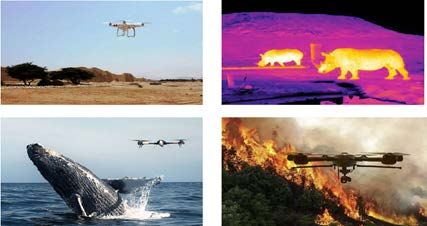
\includegraphics[width=0.5\linewidth]{imagenes/img8_ejemplos_uavs.jpg}
    \caption{Ejemplos del uso de UAVs para el monitoreo de especies en peligro de extinción y/o de su hábitat.}
    \label{fig:enter-label}
\end{figure}

\begin{table}[]
\centering
\caption{Comparación entre la propuesta de solución y el estado del arte.}
\label{tab:tabla}
\begin{tabular}{|m{0.125\textwidth}|m{0.125\textwidth}|m{0.25\textwidth}|m{0.15\textwidth}|m{0.3\textwidth}|}
\hline
Proyecto                                               & Tecnología utilizada                         & Resultados                                                                                                                                                                                  & Beneficios                                      & Limitaciones                                                                                                                            \\ \hline
Propuesta de solución este proyecto                   & WSN y enjambre de drones.                    & Brindar una mayor comprensión de la situación actual de la especie en peligro de extinción mediante un monitoreo activo, mejorando en el conocimiento tecnológico de las técnicas actuales. & Conservación de la especie.                     & Los métodos de monitoreo pueden no ser 100\% precisos, lo que puede limitar la capacidad de obtener una imagen precisa de la población. \\ \hline
Drones para el monitoreo de ballenas                   & Cámaras, análisis de exhalación.             & Datos precisos sobre tamaño, comportamiento y ubicación de ballenas, estudios de salud.                                                                                                     & Datos más precisos.                             & Dificultad para seguir a ballenas en movimientos rápidos.                                                                               \\ \hline
Uso de huellas dactilares térmicas para buscar lémures & Cámaras infrarrojas, aprendizaje automático. & Identificación de especies animales mediante huellas térmicas, análisis mediante aprendizaje automático.                                                                                    & Identificar especies.                           & Limitado a especies animales con huellas dactilares térmicas detectables.                                                               \\ \hline
Drones para la conservación de aves                    & Cámaras.                                     & Monitoreo de poblaciones de aves, estudios de comportamiento y hábitat, monitoreo de anidación .en áreas de difícil acceso                                                                  & Estudiar comportamiento y hábitat.              & Riesgo de perturbación de las aves durante el monitoreo.                                                                                \\ \hline
\end{tabular}
\end{table}


\begin{table}[]
\centering

\begin{tabular}{|m{0.125\textwidth}|m{0.125\textwidth}|m{0.25\textwidth}|m{0.15\textwidth}|m{0.3\textwidth}|}
\hline
Proyecto                                               & Tecnología utilizada                         & Resultados                                                                                                                                                                                  & Beneficios                                      & Limitaciones                                                                                                                            \\ \hline

\hline
Drones para la protección de elefantes                 & Cámaras, alertas, seguimiento.               & Monitoreo y protección de elefantes de la caza furtiva, detección de cazadores furtivos.                                                                                                    & Proteger a los elefantes de la caza furtiva.    & Necesidad de una infraestructura de vigilancia y respuesta rápida para aprovechar al máximo la detección de cazadores furtivos.         \\ \hline
Drones para la protección de rinocerontes              & Cámaras, patrullaje, seguimiento.            & Monitoreo y protección de rinocerontes de la caza furtiva, recolección de datos sobre la población de rinocerontes.                                                                         & Proteger a los rinocerontes de la caza furtiva. & Limitaciones en la cobertura de áreas extensas de terreno con drones.                                                                   \\ \hline
Protección de delfines Maui                            & Dron con inteligencia artificial.            & Obtención de datos para evitar la extinción y proteger el hábitat de los delfines Maui.                                                                                                     & Evitar la extinción de la especie.              & Dependencia de la climatología y las condiciones del mar.                                                                               \\ \hline
Protección de nidos de tortugas marinas                & Cámaras.                                     & Monitoreo y protección de nidos de tortugas marinas, identificación de amenazas y medidas de conservación.                                                                                  & Identificar posibles amenazas.                  & La interferencia humana en las playas puede aumentar el riesgo de perturbaciones en los nidos de las tortugas.                          \\ \hline

\end{tabular}
\end{table}






\begin{table}[]
\centering

\begin{tabular}{|m{0.125\textwidth}|m{0.125\textwidth}|m{0.25\textwidth}|m{0.15\textwidth}|m{0.3\textwidth}|}
\hline
Proyecto                                               & Tecnología utilizada                         & Resultados                                                                                                                                                                                  & Beneficios                                      & Limitaciones                                                                                                                            \\ \hline
Monitoreo de poblaciones de aves rapaces               & Cámaras.                                     & Monitoreo de poblaciones de aves rapaces, datos sobre su distribución y comportamiento.                                                                                                     & Obtener datos sobre su distribución.            & Restricciones en la capacidad de volar en áreas montañosas y boscosas con drones.                                                       \\ \hline
Lucha contra la caza furtiva                           & Dron con cámaras, vigilancia.                & Detección y disuasión de la caza furtiva mediante vigilancia y patrullaje de áreas protegidas.                                                                                              & Disuadir la caza furtiva.                       & Limitaciones en la capacidad de cubrir grandes áreas de terreno con drones.                                                             \\ \hline
Detección de incendios forestales                      & Dron con cámaras térmicas y sensores.        & Detección temprana de incendios forestales mediante vuelos sobre áreas forestales y detección de focos de incendio.                                                                         & Detectar focos de incendio forestal.            & Dependencia de la disponibilidad de drones y operadores para la detección temprana.                                                     \\ \hline

\end{tabular}
\end{table}


%%%%%%%%%%%%%%%%%%%%%%%%%%%
\chapter{Marco Teórico} 
\section{Especies el Peligro de Extinción}
Una especie se considera en peligro de extinción cuando se encuentra en un alto riesgo de desaparecer completamente de su hábitat natural \cite{43}. La Unión Internacional para la Conservación de la Naturaleza (IUCN, por sus siglas en inglés) ha establecido una serie de categorías de conservación para clasificar el estado de las especies en función de su riesgo de extinción, y se basa en criterios como el tamaño y tendencia de la población, la distribución geográfica, la calidad del hábitat, entre otros factores \cite{44}.\\
La IUCN utiliza las siguientes categorías de conservación:

\begin{itemize}
\item \textbf{Extinta:} Se refiere a una especie que ya no existe en la naturaleza ni en cautiverio.
\item \textbf{Extinta en estado silvestre:} se refiere a una especie que todavía existe en cautiverio pero que ya no se encuentra en su hábitat natural.
\item \textbf{En peligro crítico:} Se refiere a una especie que enfrenta un riesgo extremadamente alto de extinción en la naturaleza.
\item \textbf{En peligro:} Se refiere a una especie que enfrenta un riesgo muy alto de extinción en la naturaleza.
\item \textbf{Vulnerable:} Se refiere a una especie que enfrenta un riesgo alto de extinción en la naturaleza.
\item \textbf{Casi amenazada:} Se refiere a una especie que no cumple con los criterios para ser incluida en una categoría de mayor riesgo de extinción, pero que podría estar en peligro en el futuro.
\item \textbf{Preocupación menor:} Se refiere a una especie que no cumple con los criterios para ser incluida en una categoría de mayor riesgo de extinción.
\item \textbf{Datos insuficientes:} Se refiere a una especie que no ha sido evaluada suficientemente para determinar su estado de conservación.
\end{itemize}

\begin{figure}[h]
    \centering
    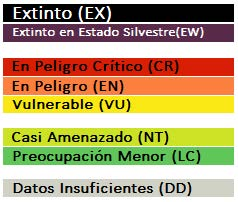
\includegraphics[width=0.4\linewidth]{imagenes/img9_categorias_iucn.jpg}
    \caption{Categorías de conservación de la IUCN.}
    \label{fig:enter-label}
\end{figure}

\noindent De acuerdo con información proporcionada por la Unión Internacional para la Conservación de la Naturaleza, actualmente se estima que alrededor de 5,200 especies están en peligro de extinción, lo que representa un porcentaje significativo de la biodiversidad. En particular, se estima que el 25\% de los mamíferos y anfibios, el 34\% de los peces, el 20\% de los reptiles y el 11\% de las aves se encuentran en peligro de extinción. Cabe destacar que estos datos se refieren únicamente a los animales vertebrados conocidos y que la cifra aumenta cuando se incluyen las especies vulnerables, es decir, aquellas que aunque no se consideran en peligro de extinción, han experimentado una rápida disminución en su población o han sufrido una considerable pérdida de su hábitat \cite{45}.

\section{Métodos Tradicionales de Monitoreo Remoto}

El monitoreo remoto se ha utilizado durante décadas para la recopilación de datos ambientales y de la presencia de animales. Los métodos tradicionales de monitoreo remoto incluyen técnicas como el uso de cámaras trampa, avistamiento visual, telemetría y radiotelemetría \cite{46}.\\
Las cámaras trampa son cámaras fotográficas que se activan mediante sensores de movimiento cuando detectan movimiento en su rango de visión. Estas cámaras se colocan en lugares estratégicos y permiten obtener imágenes de la fauna silvestre sin interferir en su comportamiento. Asimismo, las cámaras trampa pueden utilizarse para monitorear especies nocturnas o de hábitos esquivos \cite{47}.\\
El avistamiento visual consiste en la observación directa de las especies de interés por parte de un observador capacitado. Este método se utiliza para obtener información sobre el comportamiento, hábitat y distribución de las especies. Sin embargo, este método puede ser limitado por la capacidad del observador para detectar y registrar la presencia de las especies \cite{48}.\\
La telemetría es un método que utiliza dispositivos electrónicos para monitorear la ubicación y movimiento de las especies. Estos dispositivos pueden ser colocados en los animales y permiten la recolección de datos en tiempo real. La telemetría es útil para el monitoreo de especies migratorias o de comportamiento errático \cite{49}.\\
La radiotelemetría es un método de telemetría que utiliza ondas de radio para transmitir datos desde los dispositivos colocados en los animales hasta una antena receptora. Este método es útil para el monitoreo de animales que se mueven en áreas extensas o de difícil acceso \cite{50}.

\section{Enjambre de Drones}
\label{marcodrones}
Los enjambres de drones son un grupo de drones que trabajan juntos de manera coordinada con capacidad de tomar decisiones entre ellos, en lugar de estar individualmente controladas por un humano para realizar una tarea específica. Los drones de un enjambre son una tecnología se pueden clasificar según sus características y aplicaciones prácticas, tal y como se puede observar en la \hyperref[tabla2]{Tabla 8.1: Clasificación de drones según características y aplicaciones.}

\begin{table}[h]
\centering
\caption{Clasificación de drones según características y aplicaciones.}
\label{tabla2}
\resizebox{\textwidth}{!}{%
\begin{tabular}{|cccccccccccccccccccccccccc|}
\hline
\multicolumn{26}{|c|}{\cellcolor[HTML]{C0C0C0}Tamaño} \\ \hline
\multicolumn{4}{|c|}{\begin{tabular}[c]{@{}c@{}}Nano\\ \textless 30 mm\end{tabular}} &
  \multicolumn{4}{c|}{\begin{tabular}[c]{@{}c@{}}Micro\\ 30–100 mm\end{tabular}} &
  \multicolumn{4}{c|}{\begin{tabular}[c]{@{}c@{}}Mini\\ 100–300 mm\end{tabular}} &
  \multicolumn{4}{c|}{\begin{tabular}[c]{@{}c@{}}Pequeño\\ 300–500 mm\end{tabular}} &
  \multicolumn{4}{c|}{\begin{tabular}[c]{@{}c@{}}Medio\\ 500 mm–2 m\end{tabular}} &
  \multicolumn{6}{c|}{\begin{tabular}[c]{@{}c@{}}Grande\\ 2 m\end{tabular}}
  \ \\ \hline
\multicolumn{26}{|c|}{\cellcolor[HTML]{C0C0C0}Peso máximo al despegue (MTOW)} \\ \hline
\multicolumn{4}{|c|}{\textless 0.5 Kg} &
  \multicolumn{8}{c|}{0.5–5 Kg} &
  \multicolumn{8}{c|}{5–25 Kg} &
  \multicolumn{6}{c|}{\textgreater 25 Kg} \\ \hline
\multicolumn{26}{|c|}{\cellcolor[HTML]{C0C0C0}Alcance (Distancia/Tipo de Operación)} \\ \hline
\multicolumn{7}{|c|}{Corto alcance: \textless 0.5 millas} &
  \multicolumn{11}{c|}{Medio alcance: 0.5–5 millas} &
  \multicolumn{8}{c|}{Largo alcance: \textgreater 5 millas} \\ \hline
\multicolumn{7}{|c|}{\begin{tabular}[c]{@{}c@{}}Línea De Vista Visual\\ (VLOS)\end{tabular}} &
  \multicolumn{11}{c|}{Línea de Vista Visual Extendida (EVLOS)} &
  \multicolumn{8}{c|}{Fuera de la Línea de Vista Visual (BVLOS)} \\ \hline
\multicolumn{26}{|c|}{\cellcolor[HTML]{C0C0C0}Ala} \\ \hline
\multicolumn{15}{|c|}{Ala giratoria} &
  \multicolumn{10}{c|}{Ala fija} &
  Híbrido (VTOL) \\ \hline
\multicolumn{1}{|c|}{} &
  \multicolumn{14}{c|}{Multi-rotor} &
  \multicolumn{4}{c|}{} &
  \multicolumn{2}{c|}{} &
  \multicolumn{2}{c|}{} &
  \multicolumn{2}{c|}{} &
   \\ \cline{2-15}
\multicolumn{1}{|c|}{\multirow{-2}{*}{Rotores simples y dobles}} &
  \multicolumn{3}{c|}{Tricóptero} &
  \multicolumn{5}{c|}{Cuadricóptero} &
  \multicolumn{3}{c|}{Hexacóptero} &
  \multicolumn{3}{c|}{Octocóptero} &
  \multicolumn{4}{c|}{\multirow{-2}{*}{Ala baja}} &
  \multicolumn{2}{c|}{\multirow{-2}{*}{Ala media}} &
  \multicolumn{2}{c|}{\multirow{-2}{*}{Ala alta}} &
  \multicolumn{2}{c|}{\multirow{-2}{*}{Ala delta}} &
  \multirow{-2}{*}{} \\ \hline
  \multicolumn{26}{|c|}{\cellcolor[HTML]{C0C0C0}Ensamblaje} \\ \hline
  \multicolumn{8}{|c|}{Listo para Volar (RTF)} &
  \multicolumn{12}{c|}{Enlazar y Volar (BNF)} &
  \multicolumn{6}{c|}{Casi Listo para Volar (ARF)}
  \\ \hline
  \multicolumn{26}{|c|}{\cellcolor[HTML]{C0C0C0}Aplicaciones} \\ \hline
\multicolumn{4}{|c|}{Logística} &
  \multicolumn{8}{c|}{Ingeniería civil} &
  \multicolumn{8}{c|}{Asistencia en desastres} &
  \multicolumn{6}{c|}{Agricultura de precisión}
  \\ \hline
  \multicolumn{4}{|c|}{Búsqueda y rescate} &
  \multicolumn{8}{c|}{Patrimonio} &
  \multicolumn{8}{c|}{Recursos naturales} &
  \multicolumn{6}{c|}{Cumplimiento de la ley}
  \\ \hline
  \multicolumn{4}{|c|}{Gestión de la vida silvestre} &
  \multicolumn{8}{c|}{Militar} &
  \multicolumn{8}{c|}{Ocio} &
  \multicolumn{6}{c|}{Inspección industrial}
  \\ \hline
  \multicolumn{4}{|c|}{Pronóstico del tiempo} &
  \multicolumn{8}{c|}{Asistencia en desastres} &
  \multicolumn{8}{c|}{Fotografía y cine aéreo} &
  \multicolumn{6}{c|}{Arqueología}
  \\ \hline

\end{tabular}%
}
\end{table}


\noindent En un enjambre de drones, cada uno de los drones puede tener su propio conjunto de sensores (\hyperref[tabla3]{Tabla 8.2: Clasificación de sensores y dispositivos que se pueden acoplar a drones.}), habilidades y tareas, y al estar en grupo pueden trabajar en conjunto para realizar objetivos complejos que un solo dron no podría realizar por sí solo. Los enjambres de drones pueden ser programados para seguir diferentes patrones de vuelo, como vuelos en formación, vuelos en círculos o vuelos en espiral. Sumado a esto, pueden ser programados para comunicarse entre sí y con una estación base para coordinar su comportamiento y lograr los objetivos preestablecidos \cite{51}.
\newpage

% Please add the following required packages to your document preamble:
% \usepackage{multirow}
% \usepackage{graphicx}
\begin{table}[]
\centering
\caption{Clasificación de sensores y dispositivos que se pueden acoplar a drones.}
\label{tabla3}
\resizebox{\textwidth}{!}{%
\begin{tabular}{|cc|c|cl|c|c|c|}
\hline
\multicolumn{2}{|c|}{\cellcolor[HTML]{C0C0C0}Instrumento} &
  \cellcolor[HTML]{C0C0C0}Tipo de Sensor &
  \multicolumn{2}{c|}{\cellcolor[HTML]{C0C0C0}Resolución Espacial} &
  \cellcolor[HTML]{C0C0C0}Resolución Espectral &
  \cellcolor[HTML]{C0C0C0}Peso &
  \cellcolor[HTML]{C0C0C0}Costos \\ \hline
\multicolumn{1}{|c|}{\multirow{5}{*}{Sensores de imagen}} &
  RGB visibles &
  Pasivo &
  \multicolumn{2}{c|}{Muy alto1–5 cm/píxel} &
  Bajo(3 bandas) &
  Bajo\textless 0,5 kg &
  Bajo$100–$1000 \\ \cline{2-8} 
\multicolumn{1}{|c|}{} &
  Infrarrojo cercano (NIR) &
  Pasivo &
  \multicolumn{2}{c|}{Muy alto1–5 cm/píxel} &
  Bajo(3 bandas) &
  Bajo\textless 0,5 kg &
  Bajo$100–$1000 \\ \cline{2-8} 
\multicolumn{1}{|c|}{} &
  Multiespectral &
  Pasivo &
  \multicolumn{2}{c|}{Alto5–10 cm/píxel} &
  Medio(5–12 bandas) &
  Medio0,5–1 kg &
  Medio$1000–$10,000 \\ \cline{2-8} 
\multicolumn{1}{|c|}{} &
  Hiperespectral &
  Pasivo &
  \multicolumn{2}{c|}{Alto5–10 cm} &
  Alto(\textgreater 50–100 bandas) &
  Medio0,5–1 kg &
  Alto$10,000–$50,000 \\ \cline{2-8} 
\multicolumn{1}{|c|}{} &
  Térmico &
  Pasivo &
  \multicolumn{2}{c|}{Medio10–50 cm/píxel} &
  Bajo1 banda &
  Medio0,5–1 kg &
  Medio$1000–$10,000 \\ \hline
\multicolumn{1}{|c|}{\multirow{2}{*}{Sensores de alcance}} &
  Escáneres láser (LiDAR) &
  Activo &
  \multicolumn{2}{c|}{Muy alto1–5 cm/píxel} &
  Bajo1-2 bandas &
  Alto0,5–5 kg &
  Alto$10,000–$50,000 \\ \cline{2-8} 
\multicolumn{1}{|c|}{} &
  Radares de apertura sintética (SAR) &
  Activo &
  \multicolumn{2}{c|}{Medio10–50 cm/píxel} &
  Bajo1 banda &
  Alto\textgreater 5 kg &
  Muy alto\textgreater  \$50.000 \\ \hline
  \multicolumn{8}{|c|}{\cellcolor[HTML]{C0C0C0}Otros sensores y dispositivos } \\ \hline
  \multicolumn{3}{|c|}{Sensores atmosféricos} &
  \multicolumn{5}{c|}{Temperatura, presión, viento, humedad}
  \\ \hline
  \multicolumn{3}{|c|}{Sensores químicos} &
  \multicolumn{5}{c|}{Gas, geoquímica}
  \\ \hline
  \multicolumn{3}{|c|}{Sistemas de posición} &
  \multicolumn{5}{c|}{Ultrasonido, infrarrojos, radiofrecuencia, GPS}
  \\ \hline
  \multicolumn{3}{|c|}{Dispositivo de grabación} &
  \multicolumn{5}{c|}{Cámaras, micrófonos}
  \\ \hline
  \multicolumn{3}{|c|}{Dispositivos de muestreo} &
  \multicolumn{5}{c|}{Muestreo de agua, aerobiológico, microbiológico}
  \\ \hline
  \multicolumn{3}{|c|}{Otros dispositivos} &
  \multicolumn{5}{c|}{Carga, fumigación, esparcidor de semillas}
  \\ \hline
\end{tabular}%
}
\end{table}

\noindent Para implementar un enjambre de drones eficaz, es importante tener en cuenta varios factores, como la capacidad de los drones para comunicarse entre sí y de coordinar sus movimientos, la duración de la batería, la capacidad de carga, la precisión de la navegación y la capacidad de evitar obstáculos o peligros potenciales.

\section{Protocolos de Comunicación}

Los protocolos de comunicación son conjuntos de reglas y estándares que definen el intercambio de información entre dispositivos en una red de comunicaciones \cite{52}. Se pueden utilizar diversos protocolos de comunicación, según los requisitos de la aplicación y el tipo de transceptor utilizado. A continuación, se presentan algunos de los protocolos de comunicación más comunes que podrían ser utilizados en este tipo de sistema:

\begin{itemize}
    \item \textbf{IEEE 802.11 (WiFi):} Este protocolo se utiliza en redes inalámbricas de área local (WLAN) y permite la transmisión y recepción de datos a través de una conexión inalámbrica de alta velocidad. Los dispositivos que utilizan este protocolo operan en las bandas de frecuencia de 2.4 GHz y 5 GHz, y pueden transmitir datos a velocidades de hasta varios gigabits por segundo \cite{53}.
    \item \textbf{Bluetooth:} Este protocolo se utiliza para la comunicación inalámbrica de corto alcance entre dispositivos, como auriculares, altavoces y dispositivos móviles. Los dispositivos Bluetooth operan en la banda de frecuencia de 2.4 GHz y pueden transmitir datos a velocidades de hasta varios megabits por segundo \cite{54}.
    \item \textbf{Zigbee:} Este protocolo de área personal de baja potencia y alta eficiencia energética, está diseñado para permitir la comunicación entre dispositivos de bajo consumo de energía en redes de sensores y otros dispositivos inteligentes, otorgándoles una duración de batería prolongada. Los dispositivos que utilizan este protocolo operan en la banda de frecuencia de 2.4 GHz \cite{55}.
    \item \textbf{LoRaWAN:} Este protocolo ofrece una larga vida útil de la batería, una alta eficiencia energética y seguridad de red integrada para dispositivos electrónicos en áreas remotas. Se utiliza en sistemas de comunicación de largo alcance y baja potencia. Los dispositivos que utilizan este protocolo operan en las bandas de frecuencia de 868 MHz o 915 MHz \cite{56}.
    \item \textbf{MQTT:} Este protocolo se utiliza para la comunicación de mensajes entre dispositivos en una red, y es especialmente adecuado para aplicaciones IoT (Internet de las cosas) y sistemas de sensores. MQTT es un protocolo de publicación/suscripción, lo que significa que los dispositivos pueden publicar datos en un canal específico y otros dispositivos pueden suscribirse a ese canal para recibir los datos \cite{57}.
    \item \textbf{ALOHA Puro:} Este protocolo es uno de los primeros protocolos de acceso múltiple desarrollados para redes de comunicación. En ALOHA Puro, los dispositivos transmiten los datos de manera asincrónica sin sincronización previa. Si ocurre una colisión, se detecta y se realiza una retransmisión posteriormente. Este protocolo es simple pero puede presentar un alto índice de colisiones, lo que afecta la eficiencia de la comunicación \cite{58}.
    \item \textbf{ALOHA Ranurado:} Este protocolo es una mejora del protocolo ALOHA Puro y se basa en la división del tiempo en ranuras. Cada ranura se asigna a un dispositivo para transmitir sus datos, lo que reduce la probabilidad de colisiones. Sin embargo, puede haber un desperdicio de tiempo si una ranura está vacía \cite{59}.
\end{itemize}

\noindent La elección del protocolo de comunicación específico dependerá de los requisitos y las características del proyecto, aunque se considera la utilización del protocolo ALOHA Ranurado debido a su simplicidad y bajo consumo energético.

\section{Transceptores}

Los transceptores son dispositivos que se utilizan para la transmisión y recepción de señales en una red de comunicaciones inalámbrica. Estos dispositivos están diseñados para operar en una banda de frecuencia específica y utilizan un protocolo de comunicación específico para enviar y recibir datos \cite{60}. En una red inalámbrica, los transceptores se utilizan para enviar y recibir datos a través del aire. Estos dispositivos convierten la señal de datos en ondas de radio que se pueden transmitir a través del aire, y a su vez, pueden recibir señales de radio y convertirlas en datos utilizables \cite{61}. Existen varios tipos de transceptores que se utilizan comúnmente en redes inalámbricas, incluyendo:

\begin{itemize}
    \item \textbf{TransceptoresWiFi (Wireless Fidelity):} Estos dispositivos se utilizan para la conexión inalámbrica a Internet a través de una red WiFi con un radio promedio de 50 metros \cite{53}.
    \item \textbf{Transceptores Bluetooth:} Los transceptores Bluetooth se utilizan para conectar dispositivos electrónicos cercanos, con un radio promedio de 10 metros \cite{54}.
    \item \textbf{Transceptores Zigbee:} Estos dispositivos se utilizan en redes inalámbricas de sensores de baja potencia y bajo costo, contando con un radio promedio de 60 metros \cite{55}.
    \item \textbf{Transceptores LoRa (Long Range):} Estos dispositivos utilizan la modulación de espectro ensanchado para aumentar la distancia de transmisión y reducir el consumo de energía de los dispositivos de la red, estos pueden transmitir a distancias de decenas de kilómetros en condiciones óptimas \cite{56}.
    \item \textbf{Transceptores de radiofrecuencia (RF):} Estos dispositivos se utilizan en sistemas de comunicación de largo alcance, como sistemas de radio de dos vías o sistemas de telemetría. Los transceptores de RF utilizan frecuencias de radio específicas para la transmisión y recepción de datos; en un entorno sin obstáculos y sin interferencias estos cuentan con un radio de cobertura de varios cientos de metros a varios kilómetros \cite{62}.
\end{itemize}

\section{Red Inalámbrica de Sensores (WSN)}

Las redes inalámbricas de sensores (WSN) son sistemas compuestos por nodos inalámbricos que se encargan de recolectar y transmitir datos de un entorno físico a una estación base \cite{63}. Estos nodos están equipados con sensores que les permiten medir diferentes parámetros, como temperatura, humedad, presión, luz, sonido, etc.
Las WSN se utilizan en una variedad de aplicaciones, incluyendo monitoreo ambiental, control de procesos industriales, monitoreo de infraestructuras, entre otros. En particular, las WSN son muy útiles en aplicaciones de monitoreo ambiental, ya que permiten obtener información sobre el comportamiento de las especies que se encuentran en peligro de extinción, su hábitat y otros factores relevantes para su conservación.\\
El funcionamiento de una WSN se basa en la comunicación inalámbrica entre los nodos y la estación base. Los nodos inalámbricos están equipados con un transceptor que les permite comunicarse con otros nodos cercanos y con la estación base. Los datos medidos por los sensores se transmiten de nodo en nodo hasta que llegan a la estación base, que es la encargada de procesarlos y almacenarlos \cite{64}.\\
Para que una WSN sea eficiente, es necesario que se tomen en cuenta factores como el consumo energético, la escalabilidad, la robustez y la seguridad. Por ejemplo, los nodos deben ser diseñados de manera que consuman la menor cantidad de energía posible, para prolongar la duración de las baterías y reducir los costos de mantenimiento. Al mismo tiempo, es importante que la red sea escalable con el fin de poder adaptarse a diferentes tamaños de área de monitoreo y a diferentes requerimientos de densidad de sensores \cite{65}.

\section{Esquemas de Recolección}

La recolección de datos en una WSN es un proceso crítico para asegurar la precisión y eficiencia de la recopilación de información. Existen varios esquemas de recolección de datos en WSN \cite{66}, entre los que se incluyen:

\begin{itemize}
    \item \textbf{Esquema de recolección basado en eventos:} Este esquema de recolección se basa en la detección de eventos específicos en el entorno, como un cambio en la temperatura, la presencia de un objeto en movimiento, entre otros. Cuando se detecta un evento, el nodo correspondiente envía una alerta al nodo central para su posterior procesamiento.
    \item \textbf{Esquema de recolección periódica:} En este esquema, los nodos envían datos al nodo central de forma periódica. Este esquema es fácil de implementar, pero puede generar una gran cantidad de datos innecesarios si no se configura adecuadamente.
    \item \textbf{Esquema de recolección basado en consulta:} En este esquema, el nodo central realiza una consulta a los nodos para obtener información específica. Este esquema permite un mayor control sobre la cantidad de datos recopilados, ya que solo se obtiene la información relevante.
    \item \textbf{Esquema de recolección híbrido:} Este esquema combina los esquemas anteriores para obtener una mejor eficiencia en la recolección de datos. Por ejemplo, se puede utilizar el esquema basado en eventos para detectar eventos importantes y el esquema periódico para recopilar información de forma regular.
\end{itemize}

\noindent Además de estos esquemas de recolección de datos, existen técnicas para mejorar la eficiencia en la transmisión de datos, como la compresión de datos y la reducción del tamaño de los paquetes de datos enviados.

\section{Estación Base}

En un sistema de drones, la estación base es un componente crítico que permite la comunicación entre los drones y el usuario o la red central. La estación base puede ser una unidad terrestre o aérea que se encarga de controlar y supervisar el movimiento y la posición de los drones.\\
En términos de hardware, la estación base puede contar con una antena de alta ganancia que permite una comunicación bidireccional confiable con los drones. También puede tener un sistema de posicionamiento global (GPS) para rastrear la ubicación de los drones y un enlace de comunicación de datos para transmitir y recibir datos de los drones \cite{67}.\\
En cuanto a la ubicación de la estación base, depende de la aplicación específica y del área de cobertura requerida. En algunas aplicaciones, como la agricultura de precisión, la estación base puede ser una unidad fija ubicada en un lugar estratégico en el campo. En otras aplicaciones, como el monitoreo de la infraestructura de la ciudad, la estación base puede ser una unidad móvil que se desplaza por la ciudad para proporcionar cobertura en diferentes áreas \cite{68}.

\section{Almacenamiento en la Nube}

El almacenamiento en la nube, también conocido como almacenamiento en línea o almacenamiento remoto, es un modelo de almacenamiento de datos en el cual los archivos y datos se guardan en servidores remotos a los que se accede a través de Internet. Este enfoque de almacenamiento ofrece diversas ventajas y beneficios en comparación con el almacenamiento local tradicional \cite{69}. A continuación, se presentan los conceptos y aspectos clave relacionados con el almacenamiento
en la nube.

\subsection{Definición y Características del Almacenamiento en la Nube}
El almacenamiento en la nube se refiere a la práctica de guardar y gestionar datos en servidores remotos que son accesibles a través de Internet. Los datos se almacenan y mantienen en infraestructuras de centros de datos remotos, que pueden ser operados por proveedores de servicios en la nube \cite{70}. Algunas de las características importantes del almacenamiento en la nube incluyen:
\begin{itemize}
    \item \textbf{Acceso remoto:} Los usuarios pueden acceder a sus datos almacenados en la nube desde cualquier lugar y en cualquier momento, siempre que tengan una conexión a Internet.
    \item \textbf{Escalabilidad:} Los servicios de almacenamiento en la nube ofrecen la capacidad de aumentar o reducir la cantidad de almacenamiento según las necesidades del usuario, sin limitaciones físicas.
    \item \textbf{Redundancia y tolerancia a fallos:} Los proveedores de servicios en la nube implementan medidas de seguridad y copias de seguridad para garantizar la integridad y disponibilidad de los datos almacenados, minimizando la posibilidad de pérdida de datos.
    \item \textbf{Compartición y colaboración:} El almacenamiento en la nube permite compartir y colaborar en tiempo real en documentos y archivos con otras personas, facilitando el trabajo en equipo y la colaboración a distancia.
\end{itemize}

\subsection{Modelos de Servicio de Almacenamiento en la Nube}
Existen diferentes modelos de servicio de almacenamiento en la nube, que determinan la forma en que los usuarios interactúan con el almacenamiento en la nube \cite{71}. Los modelos más comunes son:
\begin{itemize}
    \item \textbf{Almacenamiento en la nube público:} En este modelo, los servicios de almacenamiento en la nube son proporcionados por proveedores externos que ofrecen almacenamiento y servicios relacionados a múltiples clientes. Los datos de los usuarios se almacenan en infraestructuras compartidas, y los usuarios pagan por el espacio de almacenamiento y los servicios utilizados.
    \item \textbf{Almacenamiento en la nube privado:} En este caso, la infraestructura de almacenamiento en la nube es propiedad y está gestionada por una organización específica, generalmente para uso interno. Proporciona mayor control y seguridad, ya que los datos se almacenan en servidores dedicados y no se comparten con otros usuarios externos.
    \item \textbf{Almacenamiento en la nube híbrido:} Este modelo combina el almacenamiento en la nube público y privado, permitiendo a las organizaciones aprovechar los beneficios de ambos enfoques. Los datos se almacenan en la nube pública y privada según su nivel de sensibilidad y requerimientos de seguridad.
\end{itemize}

\subsection{Beneficios y Desafíos del Almacenamiento en la Nube}
El almacenamiento en la nube ofrece una serie de beneficios significativos \cite{72}, como:
\begin{itemize}
    \item \textbf{Accesibilidad y disponibilidad:} Los datos almacenados en la nube están disponibles en todo momento y desde cualquier ubicación, lo que facilita el acceso y la colaboración.
    \item \textbf{Escalabilidad y flexibilidad}: Los servicios de almacenamiento en la nube permiten ajustar la capacidad de almacenamiento según las necesidades del usuario, evitando la necesidad de invertir en infraestructura adicional.
    \item \textbf{Reducción de costos:} Al utilizar el almacenamiento en la nube, los usuarios pueden evitar gastos de hardware, mantenimiento y administración de servidores locales.
    \item \textbf{Copias de seguridad y recuperación de desastres: }Los proveedores de servicios en la nube implementan medidas de copias de seguridad y recuperación de datos, lo que proporciona una mayor protección contra la pérdida de datos.
\end{itemize}

\noindent Sin embargo, también existen desafíos asociados con el almacenamiento en la nube, como la seguridad de los datos, la privacidad y la dependencia de una conexión a Internet confiable.

\subsection{Servicios y Tecnologías Populares de Almacenamiento en la Nube}
Hay una amplia gama de servicios y tecnologías disponibles en el campo del almacenamiento en la nube. Algunos de los servicios más populares incluyen:
\begin{itemize}
\item Amazon S3 (Simple Storage Service).
\item Microsoft Azure Blob Storage.
\item Google Cloud Storage.
\item Dropbox.
\item Box.
\end{itemize}

\section{Bases de Datos Relacionales y No Relacionales}

Una base de datos relacional es un tipo de sistema de gestión de bases de datos (DataBase Management System, DBMS) que organiza los datos en tablas estructuradas llamadas \textquotedbl{} tablas\textquotedbl{} o \textquotedbl{}relaciones\textquotedbl{}. Estas tablas están compuestas por filas y columnas, donde cada fila representa un registro de datos y cada columna representa un atributo o campo específico de esos registros. Algunas de las características más importantes de las bases de datos relacionales son:

\begin{itemize}
    \item \textbf{Tablas y Columnas:} Una base de datos relacional es un conjunto de tablas que contienen datos que se ajustan a categorías predefinidas. Cada tabla contiene una o varias categorías en columnas. Cada fila contiene una instancia única de datos de las categorías definidas por las columnas \cite{base2}.

\item \textbf{Clave Primaria y Clave Foránea:} Cada registro es único identificado por una clave primaria. Además, las tablas también deben tener un nombre único. Las relaciones entre distintas tablas se establecen usando claves primarias y claves foráneas \cite{base4}.

\item \textbf{Integridad de los Datos:} Este tipo de modelos mantienen una gran integridad gracias a la correctitud y completitud de la información evitando que los datos puedan ser corrompidos y que puedan añadirse nuevas entradas no válidas dentro de la base de datos \cite{base4}.

\item \textbf{Relaciones entre Tablas:} Estas relaciones permiten juntar y extraer datos de distintas tablas como si fuera una de sola. Estas relaciones se llevan a cabo usando claves primarias y claves foráneas  \cite{base4}.

\item \textbf{Índices:} Existen claves índices que permiten acceder de manera más rápida a determinados datos, pudiendo tener diferentes combinaciones para consultar algunos datos o dato en concreto \cite{base1}.
 
\end{itemize}
Ventajas de las Bases de Datos Relacionales:
 \begin{itemize}
     \item \textbf{Facilidad de Creación y Acceso: }Este tipo de base de datos son fáciles de crear y accesibles, además de tener la ventaja de ser fáciles de ampliar \cite{base2}.

\item \textbf{Gestión de Datos: }Permiten hacer un seguimiento de los inventarios, procesar transacciones de comercio electrónico, gestionar grandes cantidades de información de clientes y mucho más \cite{base2}.

\item \textbf{SQL: }Todas las bases de datos relacionales funcionan con un gestor que permite extraer información usando lo que se conoce como SQL (Structured Query Language). Esto permite que haya una unificación y que una base de datos puede ser usada con distintos gestores \cite{base4}.
\item \textbf{Simplicidad:} Uno de sus puntos fuertes es su sencillez de uso. El SQL es un lenguaje que se parece mucho al lenguaje natural humano, con lo que, con poco tiempo se puede aprender a manejar este tipo de gestores \cite{base4}.
\end{itemize}
Por otra parte, una base de datos no relacional, también conocida como base de datos NoSQL (No Structured Query Language o No Solo SQL), es un tipo de sistema de gestión de bases de datos diseñado para almacenar y administrar datos de manera más flexible a datos que es muy difícil crear una relación entre los datos \cite{base5}. Algunas de las características más importantes de las bases de datos NoSQL:

\begin{itemize}
    \item \textbf{Organización de Datos:} En las bases de datos relacionales, la información se organiza de manera estructurada en tablas. Sin embargo, en las bases de datos no relacionales, la información no necesariamente se organiza en estructuras fijas como las tablas. En cambio, utilizan diversas estructuras de datos flexibles, como pares de clave-valor o grafos, para el almacenamiento y la recuperación de datos \cite{nbase2} \cite{nbase3}.

\item \textbf{Esquemas Flexibles:} Las bases de datos no relacionales suelen ofrecer esquemas flexibles, lo que permite un desarrollo más rápido y más iterativo. Son ideales para datos semiestructurados y no estructurados \cite{nbase4}.

\item \textbf{Arquitectura Distribuida:} Estas bases de datos ofrecen una arquitectura distribuida que permite almacenar información en casos en los que las bases de datos relacionales no son capaces de ofrecer el rendimiento y la escalabilidad necesarios \cite{nbase3}.

\item \textbf{Alto Rendimiento:} Las bases de datos NoSQL están optimizadas para modelos de datos específicos y patrones de acceso que permiten un mayor rendimiento que el intento de lograr una funcionalidad similar con bases de datos relacionales \cite{nbase4}.

\item \textbf{Escalabilidad:} Las bases de datos NoSQL generalmente están diseñadas para escalar usando clústeres distribuidos de hardware en lugar de escalar añadiendo servidores caros y sólidos. Algunos proveedores de la nube manejan estas operaciones en segundo plano, como un servicio completamente administrado \cite{nbase4}.

\item \textbf{Tipos de Bases de Datos NoSQL:} Existen diferentes tipos de bases de datos no relacionales, en función del método que emplean para almacenar la información. Algunos ejemplos son las bases de datos de clave-valor, las bases de datos documentales, las bases de datos orientadas a grafos, las bases de datos tabulares y las bases de datos orientadas a objetos \cite{nbase3}.

\item \textbf{Compatibilidad con Lenguajes de Consulta:} Muchas bases de datos NoSQL no usan el lenguaje SQL para consultas, o lo usan como un lenguaje secundario. Esto se debe a que las bases de datos NoSQL están diseñadas para manejar grandes volúmenes de datos y no siempre se ajustan bien a las consultas complejas que se pueden realizar con SQL \cite{nbase2}.

\item \textbf{Alto Soporte de la Comunidad:} A diferencia de las bases de datos relacionales, las bases de datos NoSQL suelen tener un soporte de la comunidad más fuerte, ya que son relativamente más nuevas y están en constante evolución \cite{nbase2}.
 
\end{itemize}

\newpage

%%%%%%fin del archivo
\endinput 